\documentclass[10pt]{beamer}

\usepackage[utf8]{inputenc}
\usepackage[spanish, es-tabla]{babel}

\usetheme{metropolis}
\usepackage{appendixnumberbeamer}

\usepackage{booktabs}
\usepackage[scale=2]{ccicons}

\usepackage{pgfplots}
\usepgfplotslibrary{dateplot}

\usepackage{graphicx}

\usepackage{xspace}
\newcommand{\themename}{\textbf{\textsc{metropolis}}\xspace}

\title{Vault7 WikiLeaks y Wannacry}
\date{\today}
\institute{Ingeniería de Servidores 2017 \\
	Universidad de Granada}

\begin{document}

\maketitle

\begin{frame}{Contenidos}
  \setbeamertemplate{section in toc}[sections numbered]
  \tableofcontents[hideallsubsections]
\end{frame}

\section{Releases Vault-7}

\begin{frame}{WikiLeaks y Vault 7}
	\pause
	\begin{center}
		
\includegraphics[scale=0.2]{./Imagenes/vault7.jpg}
	\end{center}
	\pause
	\begin{itemize}
		\item ¿Qué es WikiLeaks?
		\pause
		\item ¿Qué es Vault 7?
		\pause
		\item ¿Por qué nos interesa tanto a los usuarios como a los administradores de sistemas?
	\end{itemize}
\end{frame}

\begin{frame}{Dark Matter}
	\pause
	\begin{center}
		
\includegraphics[scale=0.25]{./Imagenes/dark-matter.jpg}
	\end{center}
	\pause
	\begin{itemize}
		\item 23 de Marzo de 2017
		\pause
		\item Infección permanente del firmware de dispositivos y ordenadores de Apple.
		\pause
		\item Permite inyección de código malicioso a través del firmware y persistentes al reinicio.
		\pause
		\item Se pueden infectar dispositivos de arranque EFI/UEFI para ejecutar código malicioso al inicio de la máquina.
	\end{itemize}	
\end{frame}

\begin{frame}{Marble Framework}
	\pause
	\begin{center}
		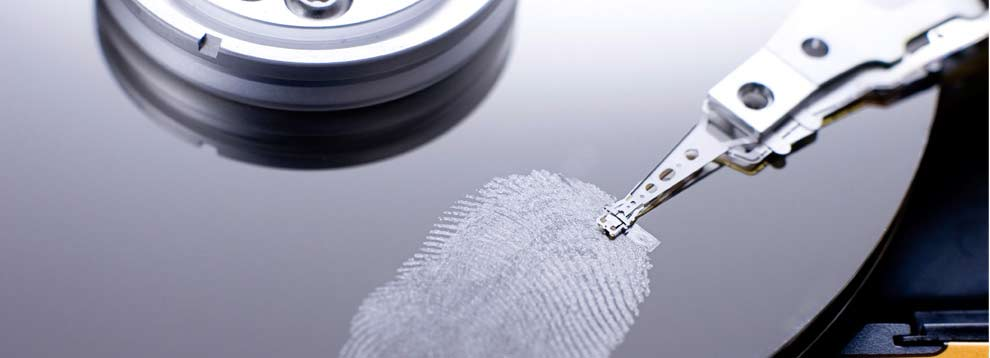
\includegraphics[scale=0.25]{./Imagenes/marble-framework.jpg}
	\end{center}
	\pause
	\begin{itemize}
		\item 31 de Marzo de 2017
		\pause
		\item Herramienta para ocultar datos ante un análisis forense informático.
		\pause
		\item Hace esto escondiendo el malware creado por la CIA e introduciendo idiomas variados y con distintas codificaciones con la intención de confundir a analistas y antivirus.
	\end{itemize}
\end{frame}

\begin{frame}{Grasshopper}
	\pause
	\begin{center}
		
\includegraphics[scale=0.3]{./Imagenes/grasshopper.jpg}
	\end{center}
	\pause
	\begin{itemize}
		\item 7 de Abril de 2017
		\pause
		\item Plataforma de creación de malware para Windows.
		\pause
		\item Crea un lenguaje de módulos sencillos para confeccionar malware aprovechando vulnerabilidades conocidas.
	\end{itemize}
\end{frame}

\begin{frame}{Hive}
	\pause
	\begin{center}
		
\includegraphics[scale=0.3]{./Imagenes/hive.jpg}
	\end{center}
	\pause
	\begin{itemize}
		\item 14 de Abril de 2017
		\pause
		\item Monitorización de usuarios y obtención de información gracias a una plataforma back-end
		\pause
		\item Utiliza HTTPS con una interfaz y consola interactiva.
		\pause
		\item Emplea dominios e IPs específicas para cada usuario que quiera ser monitorizado.
	\end{itemize}
\end{frame}

\begin{frame}{Weeping Angel}
	\pause
	\begin{center}
		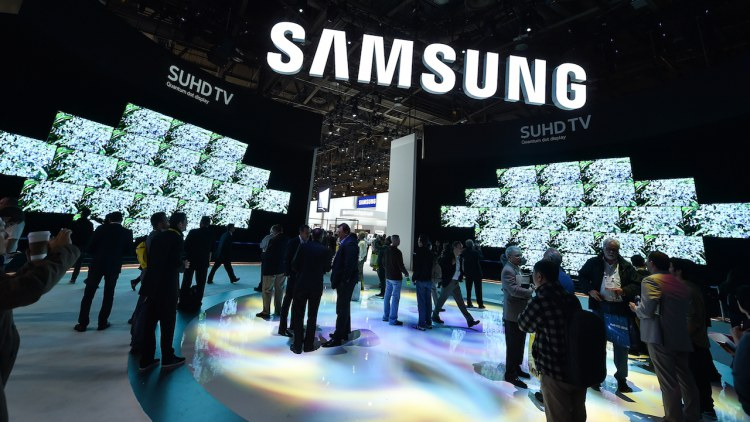
\includegraphics[scale=1.2]{./Imagenes/weeping-angel.jpg}
	\end{center}
	\pause
	\begin{itemize}
		\item 21 de Abril de 2017
		\pause
		\item Herramienta para espiar a usuarios a través de vulnerabilidades y puertas traseras de la serie F de televisores de Samsung.
		\pause
		\item Esta serie de televisiones tienen micrófono, usado en los espionajes.
	\end{itemize}
\end{frame}

\begin{frame}{Scribbles}
	\pause
	\begin{center}
		
\includegraphics[scale=0.5]{./Imagenes/scribbles.png}
	\end{center}
	\pause
	\begin{itemize}
		\item 28 de Abril de 2017
		\pause
		\item Se aprovecha de marcas de agua que monitorizan quién está leyendo un documento.
		\pause
		\item Se comunican con servidores preparados para recibir datos de este tipo.
		\pause
		\item Afecta a documentos generados con las versiones de Microsoft Office 1997-2016.
	\end{itemize}
\end{frame}

\section{Wannacry}

\begin{frame}{¿Qué es Wannacry?}
	\pause
	\begin{center}
		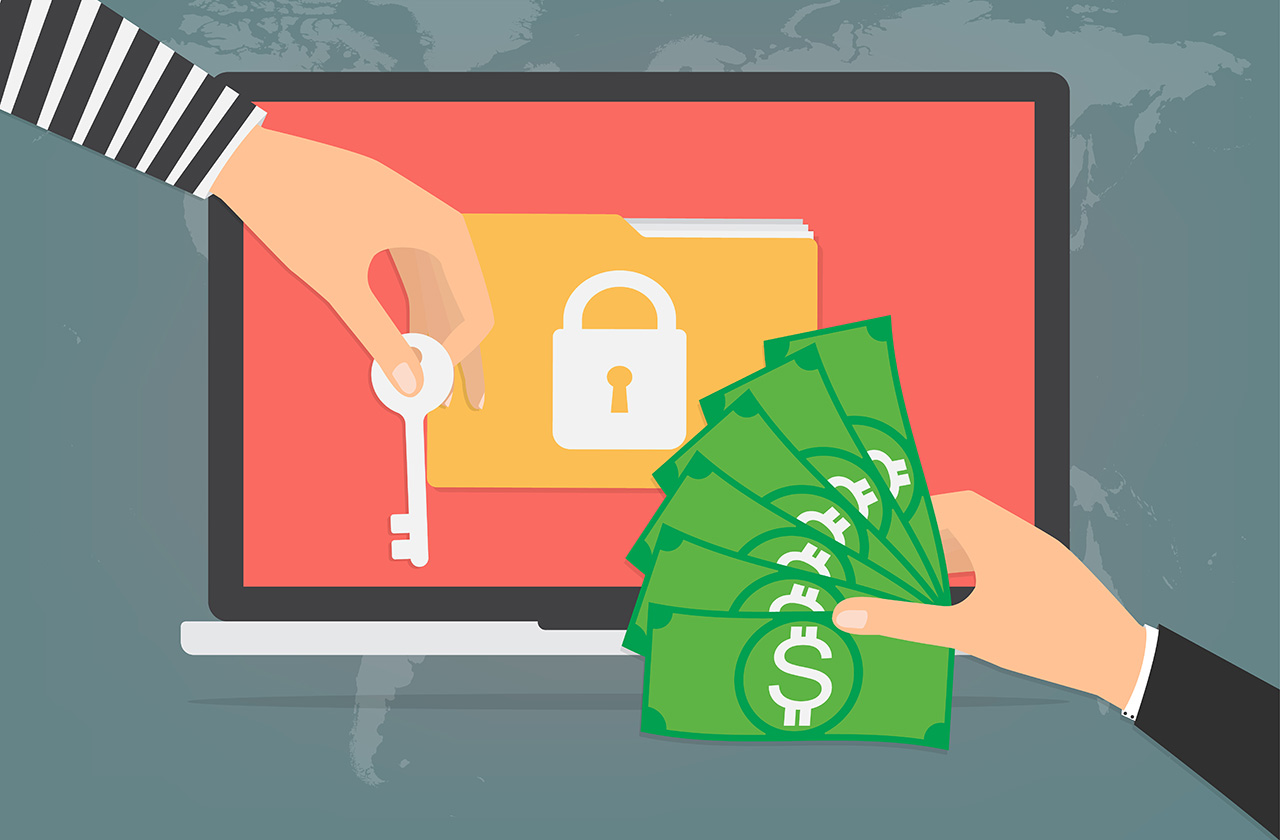
\includegraphics[scale=0.15]{./Imagenes/wannacry-1.jpg}
	\end{center}
	\pause
	\begin{itemize}
		\item Wannacry es un ransomware.
		\pause
		\item ¿Cómo se ha infectado por primera vez?
		\pause
		\item Las plataformas afectadas son las máquinas Windows en sus diferentes versiones.
	\end{itemize}
\end{frame}

\begin{frame}{¿Cómo funciona?}
	\pause
	\begin{center}
		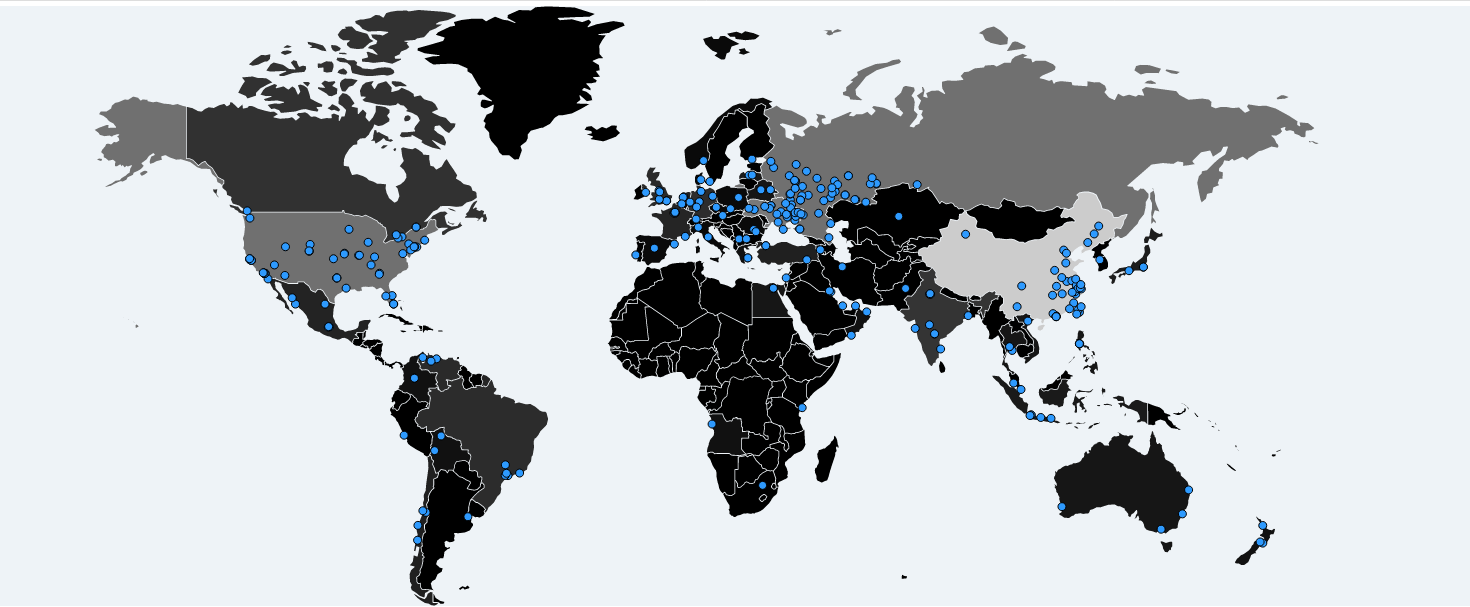
\includegraphics[scale=0.15]{./Imagenes/wannacry-2.png}
	\end{center}
	\pause
	\begin{itemize}
		\item ¿Qué medidas de seguridad hemos tomado para probar el malware?
		\pause
		\item ¿Como infecta usando SMB?
		\pause
		\item ¿Cómo encripta los archivos y cómo se recuperan si pagas?
	\end{itemize}
\end{frame}

\begin{frame}{Análisis forense del malware}
	\pause
	\begin{center}
		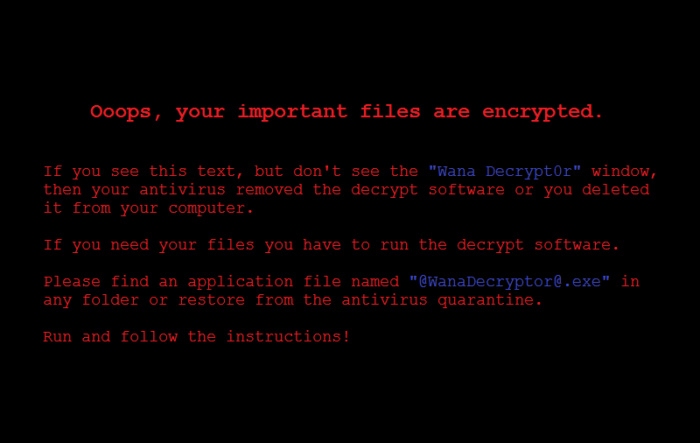
\includegraphics[scale=0.25]{./Imagenes/wannacry-3.jpg}
	\end{center}
	\pause
	\begin{itemize}
		\item Strings sobre el ejecutable.
		\pause
		\item KillSwitch del malware.
		\pause
		\item Estudio del malware sobre una máquina virtual.
	\end{itemize}
\end{frame}

\begin{frame}[standout]{Preguntas}
	\begin{center}
		
\includegraphics[scale=0.45]{./Imagenes/chema-alonso.jpg}
	\end{center}
\end{frame}

\end{document}
